	%Teniendo la variable cuantitativa discreta como independiente, se tienen varios
	%valores de y_{i} para un valor de x_{j}, realice los siguientes puntos
	\begin{enumerate}
		\item Calcular:
			\begin{itemize}
			\item Promedios de $y_{i}$ que corresponden a un $x_{j},\ \forall\ i,j$ \\ \\
			En nuestro caso, tomamos $y_i = $ A~nos que lleva en la universidad (discreta) y por conveniencia tomamos $x_j = $ Prioridad Acad\'emica.\\
			Entonces, calculamos los promedios de $x_j$ para cada $y_i$ y obtenemos la siguiente tabla:\\ \\
			\begin{tabular}{c|c}
			\hline
			A\~nos en la Universidad & Promedio Prioridad Acad\'emica \\
			\hline
			1 & 5497,36 \\
			\hline
			2 & 5920,04 \\
			\hline
			3 & 6359,83 \\
			\hline
			4 & 5870,86 \\
			\hline
			5 & 5327,38 \\
			\hline
			6 & 5703,80 \\
			\hline
			7 & 0000,00 \\
			\hline
			8 & 5083,33 \\
			\hline
			\end{tabular}
			\item Covarianza: $ -2500.714 $
			\item Coeficiente de correlaci\'on: $ -0.4989711 $
			\item Coeficientes de la recta de regresi\'on: $y\ =\ b_{1} \cdotp x\ +\ b_{0}$, $y\ =\ -416.8 \cdotp x\ +\ 6845.9 $
			\item Desviaci\'on t\'ipica generalizada: $1915$
			\item Media: 4970,32791
			\item Varianza de los errores: $Error\ b_{1}\ =\ 295.5$, $Error\ b_{0}\ =\ 1492.3 $
			\end{itemize}
		\item Gr\'aficos:
			\begin{itemize}
			\item Dispersi\'on con la recta de regresi\'on:
			\begin{center}
			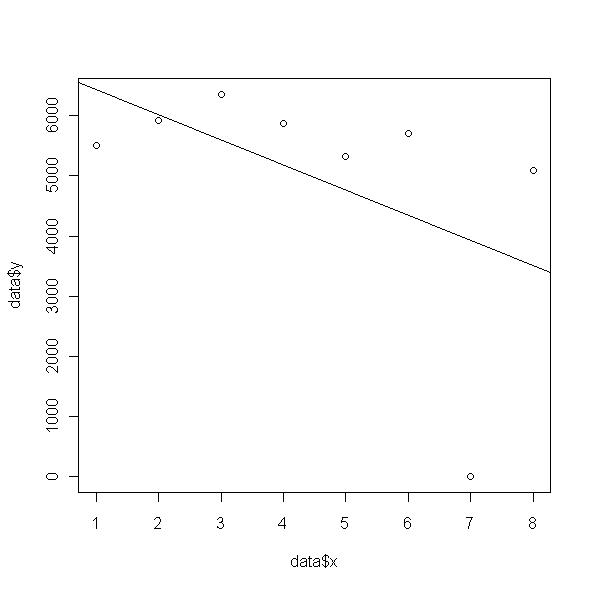
\includegraphics[width=4in,height=4in]{images/grafico_dispersion_optativo}
			\end{center}
			\item Diagrama de caja:
			\begin{center}
			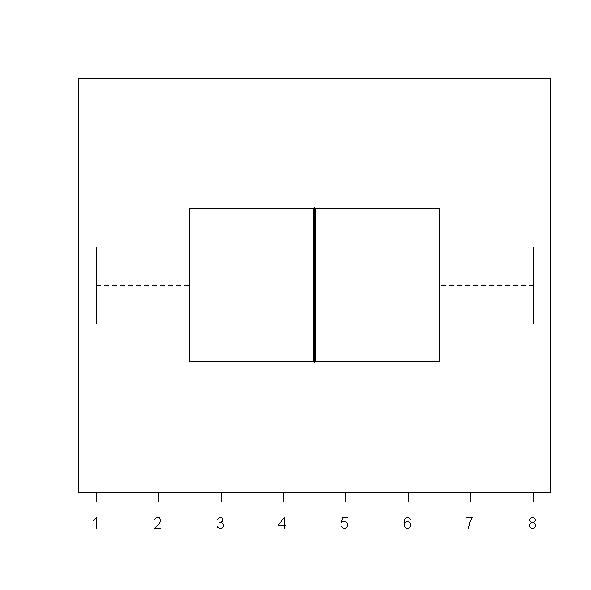
\includegraphics[width=4in,height=4in]{images/boxplot}
			\end{center}
			\item Histograma de los errores:
			\begin{center}
			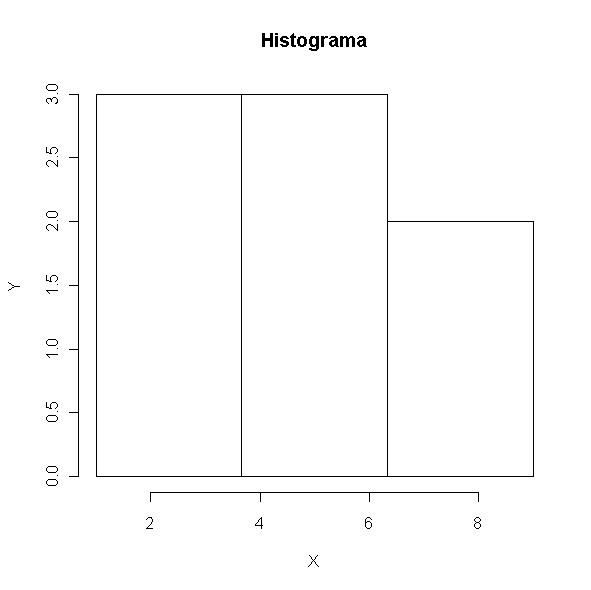
\includegraphics[width=4in,height=4in]{images/histograma}
			\end{center}
			\end{itemize}
		\item Conclusi\'on:
			Como podemos observar en la recta de regresi\'on, al parecer si existe una relaci\'on entre las variables,
			espec\'ificamente una relaci\'on inversamente proporcional entre los a~nos de estad\'ia en la Universidad
			T\'ecnica Federico Santa Mar\'ia y la Prioridad Acad\'emica del alumno. Posiblemente porque seg\'un est\'a
			dada la ecuaci\'on para calcular este coeficiente, es mucho mas dificil para el alumno aumentarlo que disminuirlo,
			lo cual queda demostrado, por la cantidad de gente que tiene que irse de la universidad por tener una prioridad
			muy baja, ya que los ramos de los primeros a\~nos son claves para poder tener una buena prioridad de base, tomando
			en cuenta que mas adelante el grado de dificultad de los ramos aumenta y hay mucha m\'as probabilidad de reprovar
			algun ramo y como los cr\'editos no son tantos, subir la prioridad acad\'emica es a\'un mas dificil.
	\end{enumerate}
